% @Author: AnthonyKenny98
% @Date:   2020-04-09 10:22:31
% @Last Modified by:   AnthonyKenny98
% @Last Modified time: 2020-04-09 21:02:37
\textit{Philosophy 4}, written in 1903 by Mr. Owen Wister of the Class of 1882 (founder of the Western literary genre), recounts the antics of two Harvard students and their last minute attempts to study (or avoid studying) for a Philosophy exam for which they are hopelessly unprepared. Similarly, this section details the process of building a RISC-V processor, by far the most intricate engineering challenge of this Thesis, and a task for which I was unsure of my preparedness. As such, this processor was named \textbf{Philosophy V}; both in reference to the RISC-V ISA for which it was designed, and to the fact that the process of its implementation at times seemed very much like a sequel to Mr. Wister's novel.
    

    \subsection{RV32I Implementation}
        Figure \ref{fig:philv_rv32i} 

        % @Author: AnthonyKenny98
% @Date:   2020-04-09 20:56:24
% @Last Modified by:   AnthonyKenny98
% @Last Modified time: 2020-04-10 06:41:52
\begin{figure}[H]
\begin{center}
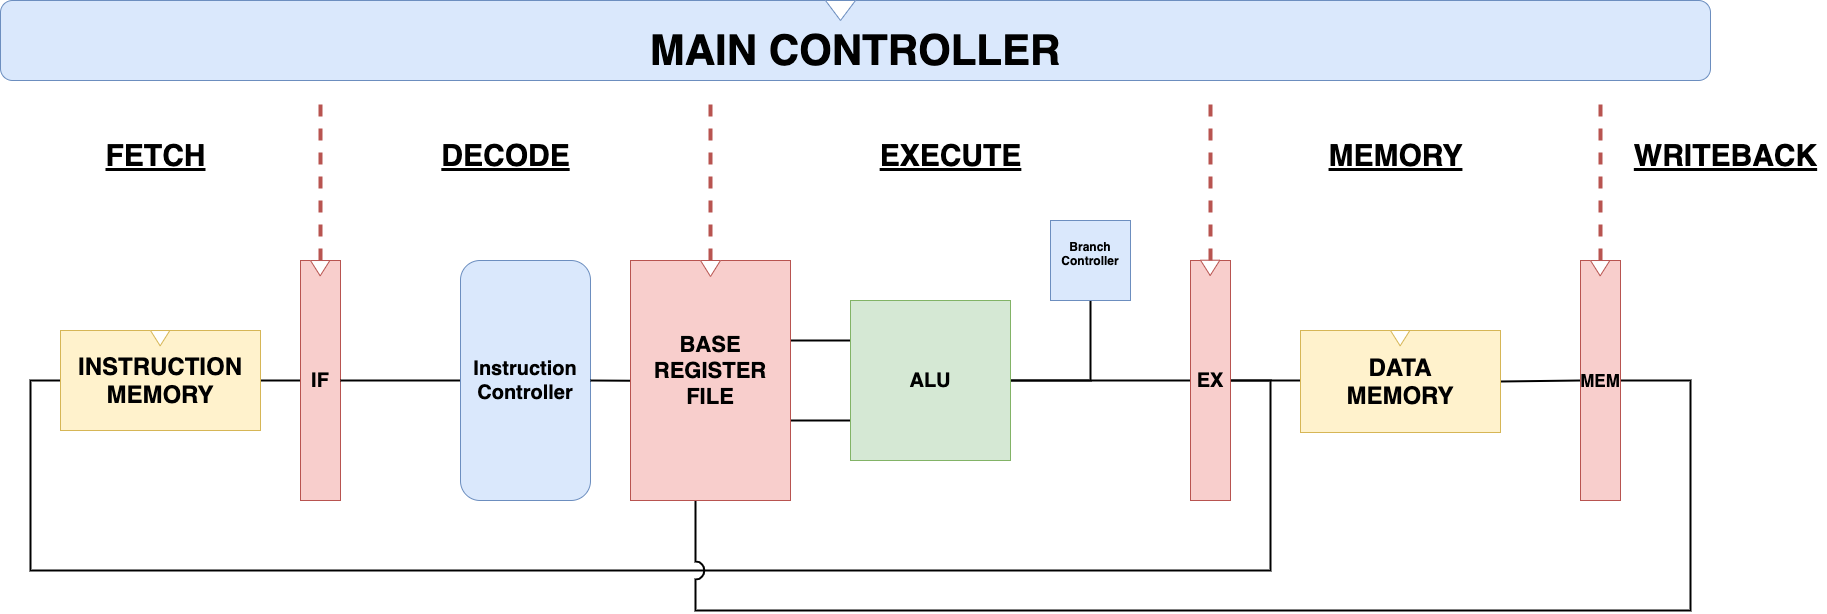
\includegraphics[width=\textwidth]{chapters/chapter4/img/philv_rv32i.png}
\mycaption{Simplified Schematic of the RV32I PhilosophyV Core}{}
\label{fig:philv_rv32i}
\end{center}
\end{figure}

        Appendix \ref{section:philv_appendix_rv32i_core} provides a detailed schematic of the PhilosophyV processor.
        

    \subsection{RV32I\_Xedgcol Implementation}
        \todo[inline]{Process of implementing honeybee into PhilV.}

    \subsection{Verification and Analysis}
        \todo[inline]{Comparative Performance Analysis of baseline and extended PhilV Core}